
\documentclass{template/socthesis}

\usepackage[left=35mm, right=30mm]{geometry}
\usepackage{subcaption}

\graphicspath{ {./images/} }

\addbibresource{sources.bib}

% Title Page
\titlesk{BrailleFeeder - pomôcka pre zrakovo postihnutých}
\school{Stredná odborná škola}
\address{Športová 675, 916 01 Stará Turá}
\author{Juraj Kulich}
\mentor{}
\field{18}


\begin{document}
	
\maketitle
\makecopyrightstatement{V Novom Meste nad Váhom}
\makethanks{Ďakujem svojmu spolužiakovi Romanovi Mariančíkovi za obetavú pomoc, podmetné  pripomienky a nekonečnú trpezlivosť, ktorú mi počas práce poskytoval.}

\tableofcontents

\chapter*{Úvod}
\addcontentsline{toc}{chapter}{Úvod}
V roku 2015 malo približne 441 milónov ľudí zrakové postihnutie. Z toho bolo 36 milónov ľudí slepých \cite{bourne2017magnitude}. Takíto ľudia môžu použiť namiesto klasického textu Braillovo písmo, avšak drvivá väčšina pomenovaní a názvov je v klasickom písme. Takisto nikde nenájdeme noviny v Braillovom písme.

TODO

Aplikácia beží na systéme Android. Na tomto systéme beží celosvetovo už cez 2 miliardy aktívnych zariadení \cite{ng_2017}. Náš systém beží na minipočítači, na ktorom je platforma Android Things, ktorá je taktiež založená na Androide. Z toho dôvodu môžeme našu aplikáciu implementovať aj na mobilné zariadenia, na ktoré však nemôžeme pripojiť periférie a tak je funkčnosť obmedzená.
\newpage
\chapter*{Cieľ práce}
\addcontentsline{toc}{chapter}{Cieľ práce}
\newpage
\chapter*{Metodika práce}
\addcontentsline{toc}{chapter}{Metodika práce}
\newpage
\chapter{Braillovo písmo}
Braillovo písmo je druh písma určeného pre nevidiacich a slabozrakých. Funguje na princípe vyvýšených bodov, ktoré sa dajú čítať hmatom.
\section{Braillovo písmeno}
Jedno písmeno Braillovho písma tvorí mriežka šiestich bodov usporiadaných do obdĺžnika 2x3. Písmeno Braillovho písma je vo veľkosti rozmeru ukazováka, keďže na brušku ukazováka je najcitlivejšá prah hmatu.

Naše písmeno je však z dôvodu elektronického a veľmi lacného prevedenia(približne 19) väčšie ako je národná norma. Napriek tomu je však použiteľné. Na porovnanie, výrobná cena štandardizovaného článku je okolo 30 a je nemožné sa k takým kusom dostať.
\newpage
\chapter{Android Things OS}
Android Things je zjednodušená verzia operačného systému Android prispôsobená pre IoT zariadenia. Je navrhnutý tak aby fungoval v inteligentných zariadeniach, napríklad termostatoch alebo kamerách.

\section{IoT - Internet of Things}
Internet of Things, v preklade internet vecí, v informatike označuje sieť fyzických zariadení, vozidiel, domácich spotrebičov a ďalších zariadení, ktoré môžu byť vybavené elektronikou, softvérom, senzormi a sieťovou konektivitou, ktorá týmto zariadeniam umožňuje vzájomné prepojenie a výmenu dát. \cite{karimi2013internet}
\section{Android OS}
Android je open source operačný systém pre mobilné zariadenia vyvíjaný spoločnosťou Google. Je postavený na jadre Linuxu. V tejto kapitole si ukážeme vlastnosti  a princípy tohto systému a spôsoby tvorby aplikácii pre tento systém.

\subsection{Základné princípy}
\subsubsection{Architektúra systému Android}

Architektúra systému Android je rozdelená do niekoľkých vrstiev (Obr. 2.1) pričom každá vrstva využíva služby vrstvy pod ňou. 
\begin{center}
	\begin{figure}[htp]
		\caption{Architektúra systému Android}
		\centering
		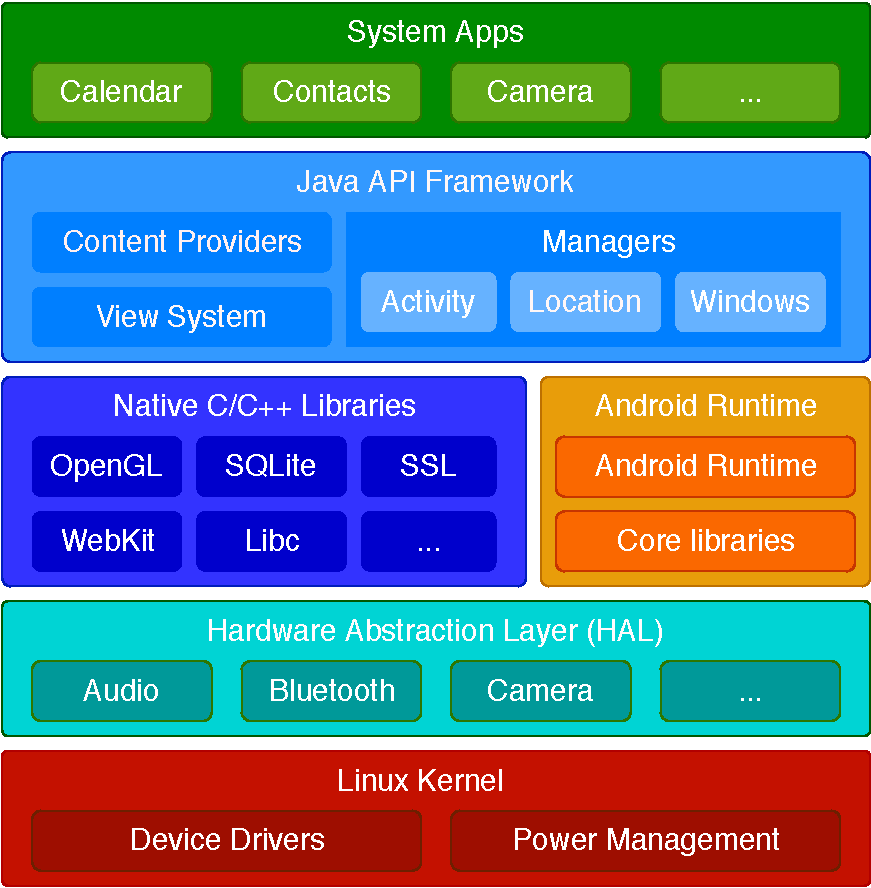
\includegraphics[scale=0.60]{android_architecture}
	\end{figure}
\end{center}

Vrstvy začiatkom od spodnej sú \cite{gandhewar2010google}:
\begin{itemize}
	\item Linux Kernel -- Jadro systému, ktoré poskytuje systémové služby ako sú bezpečnosť, správa pamäte, procesov, sietí a driverov. Slúži taktiež ako abstraktná vrstva medzi hardvérom a softvérom.  
	\item Hardware Abstraction Layer (HAL) -- Hardvérová abstraktná vrstva, ktorá poskytuje štandardné rozhrania vyššej vrstve. Skladá sa z rôznych knižníc, z ktorej kazdá implementuje rozhranie pre špecifický komponent, napríklad kameru alebo Bluetooth.
	\item Libraries -- Knižnice písané v jazykoch C a C++. Sú volané cez Java rozhranie. Obsahujú knižnice pre 2D alebo 3D grafiku, kodeky ako MP3 alebo MPEG-4, SQL databázu alebo WebKit - renderovacie jadro pre prehliadače. 
	\item Android Runtime --
	\item Java API Framework --
	\item System Applications --
\end{itemize}
\newpage

\printbibliography[title=Zoznam použitej literatúry]

\end{document}          
